\documentclass{exam}

\usepackage{units} 
\usepackage{graphicx}
\usepackage[fleqn]{amsmath}
\usepackage{cancel}
\usepackage{float}
\usepackage{mdwlist}
\usepackage{booktabs}
\usepackage{cancel}
\usepackage{polynom}
\usepackage{caption}
\usepackage{fullpage}
\usepackage{comment}
\usepackage{enumerate}
\usepackage{xfrac}

\newcommand{\dg}{\ensuremath{^\circ}} 
\everymath{\displaystyle}

\printanswers
\excludecomment{comment}

\ifprintanswers 
  \usepackage{2in1, lscape} 
\fi

\author{}
\date{October 30, 2013}
\title{Math 142 \\ Homework Nine}

\begin{document}

  \maketitle

  \section{Homework}
  Section 6.3: 1-15, 21-26, 33-46, 52-54, 65-66

  \section{Extra Credit}
  Section 6.3: 57 and 58

  \ifprintanswers
    \begin{description}
      \item[57]
        The area of the entire circle is: 
        \[
          A_{circle} = \pi 2^2 = 4 \pi
        \]

        The sector is one third of the circle or: 
        \[
          A_{sector} = \frac{4 \pi}{3}
        \]

        The area of the triangle is: 
        \[
          A_{triangle} = \frac{1}{2} \cdot 2^2 \sin 120 \dg = \sqrt{3}
        \]

        The area of the shaded region is the difference:
        \[
          A_{shaded} = A_{sector} - A_{triangle} = \frac{4 \pi}{3} - \sqrt{3} \approx \boxed{ 2.457 }
        \]

      \item[58]
        The area of the entire circle is: 
        \[
          A_{circle} = \pi 12^2 = 144 \pi
        \]

        The area of the sector is: 
        \[
          A_{sector} = \frac{1}{2} r^2 \theta = 24 \pi
        \]

        The area of the triangle is: 
        \[
          A_{triangle} = \frac{1}{2} \cdot 12^2 \sin \frac{\pi}{3} = 36 \sqrt{3}
        \]

        The area of the unshaded region is the difference between the area of the sector and the area of the triangle:
        \[
          A_{unshaded} = A_{sector} - A_{triangle} = 24 \pi - 36 \sqrt{3} \approx 13.04
        \]

        The area of the shaded region is the difference between the area of the circle and the area of the unshaded
        region:
        \[
          A_{shaded} = A_{circle} - A_{unshaded} \approx 144 \pi - 13.04 \approx \boxed{ 439.34 }
        \]
      \end{description}

  \fi

  \ifprintanswers
    \pagebreak
  \fi

  \section{Review}
  Find the period and graph:

  \begin{enumerate}
    \item $y = \tan 2 \pi x$
      \ifprintanswers
        \[
          p = \frac{\pi}{2 \pi} = \frac{1}{2}
        \]
        
        \begin{figure}[H]
          \centering
          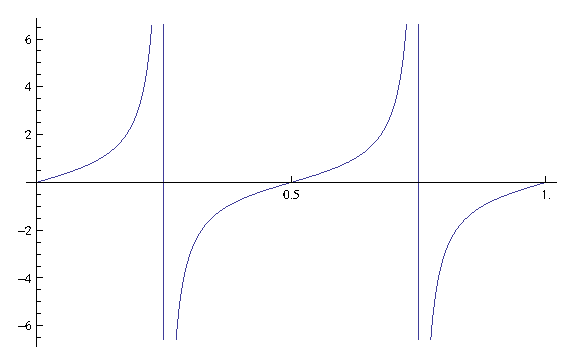
\includegraphics[scale=0.7]{review1.eps}
          \caption{Review One}
        \end{figure}
      \fi

    \item $y = 2 \sec 3x$
      \ifprintanswers
        \[
          p = \frac{2 \pi}{3}
        \]
        
        \begin{figure}[H]
          \centering
          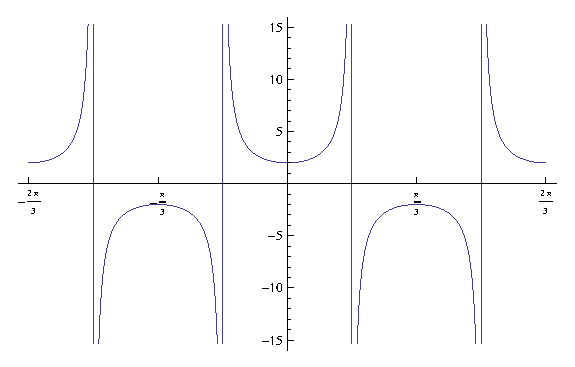
\includegraphics[scale=0.7]{review2.eps}
          \caption{Review Two}
        \end{figure}
      \fi

  \end{enumerate}

  \ifprintanswers

  \pagebreak

    \section{Section 6.3}

    \begin{description}

      \item[1] 
        \begin{enumerate}[(a)]
          \item $180 \dg - 150 \dg = \boxed{ 30 \dg }$
          \item $360 \dg - 330 \dg = \boxed{ 30 \dg }$
          \item $0 \dg - (-30 \dg) = \boxed{ 30 \dg }$
        \end{enumerate}

      \item[2] 
        \begin{enumerate}[(a)]
          \item $180 \dg - 120 \dg = \boxed{ 60 \dg }$
          \item $180 \dg - 210 \dg = \boxed{ 30 \dg }$
          \item $780 \dg - 720 \dg = \boxed{ 60 \dg }$
        \end{enumerate}

      \item[3] 
        \begin{enumerate}[(a)]
          \item $225 \dg - 180 \dg = \boxed{ 45 \dg }$
          \item $810 \dg - 720 \dg = \boxed{ 90 \dg }$
          \item $180 \dg - 105 \dg = \boxed{ 75 \dg }$
        \end{enumerate}

      \item[4] 
        \begin{enumerate}[(a)]
          \item $180 \dg - 99 \dg = \boxed{ 81 \dg }$
          \item $199 \dg - 180 \dg = \boxed{ 19 \dg }$
          \item $360 \dg - 359 \dg = \boxed{ 1 \dg }$
        \end{enumerate}

      \item[5] 
        \begin{enumerate}[(a)]
          \item $\frac{12 \pi}{4} - \frac{11 \pi}{4} = \boxed{ \frac{\pi}{4} }$
          \item $\frac{12 \pi}{6} - \frac{11 \pi}{6} = \boxed{ \frac{\pi}{6} }$
          \item $\frac{12 \pi}{3} - \frac{11 \pi}{3} = \boxed{ \frac{\pi}{3} }$
        \end{enumerate}

      \item[6] 
        \begin{enumerate}[(a)]
          \item $\frac{4 \pi}{3} - \frac{3 \pi}{3} = \boxed{ \frac{\pi}{3} }$
          \item $\frac{33 \pi}{4} - \frac{32 \pi}{4} = \boxed{ \frac{\pi}{4} }$
          \item $\frac{24 \pi}{6} - \frac{23 \pi}{6} = \boxed{ \frac{\pi}{6} }$
        \end{enumerate}

      \item[9]
        \[
          \sin 150 \dg = \sin 30 \dg = \boxed{ \frac{1}{2} }
        \]

      \item[10]
        \[
          \sin 225 \dg = - \sin 45 \dg = \boxed{ - \frac{\sqrt{2}}{2} }
        \]

      \item[11]
        \[
          \cos 135 \dg = - \cos 45 \dg = \boxed{ - \frac{\sqrt{2}}{2} }
        \]

      \item[12]
        \[
          \cos (-60 \dg) = \cos 60 \dg = \boxed{ \frac{1}{2} }
        \]

      \item[13]
        \[
          \tan (-60 \dg) = - \tan 60 \dg = \boxed{ - \sqrt{3} }
        \]

      \item[14]
        \[
          \sec (300 \dg) = \sec 60 \dg = \boxed{ 2 }
        \]

      \item[15]
        \[
          \csc (-630 \dg) = \csc 90 \dg = \boxed{ 1 }
        \]

      \item[21]
        \[
          \sin \frac{2 \pi}{3} = \sin \frac{\pi}{3} = \boxed{ \frac{\sqrt{3}}{2} }
        \]

      \item[22]
        \[
          \sin \frac{5 \pi}{3} = - \sin \frac{\pi}{3} = \boxed{ - \frac{\sqrt{3}}{2} }
        \]

      \item[23]
        \[
          \sin \frac{3 \pi}{2} = - \sin \frac{\pi}{2} = \boxed{ - 1 }
        \]

      \item[24]
        \[
          \cos \frac{7 \pi}{3} = \cos \frac{\pi}{3} = \boxed{ \frac{1}{2} }
        \]

      \item[25]
        \[
          \cos \frac{-7 \pi}{3} = \cos \frac{\pi}{3} = \boxed{ \frac{1}{2} }
        \]

      \item[26]
        \[
          \tan \frac{5 \pi}{6} = - \tan \frac{\pi}{6} = \boxed{ - \frac{\sqrt{3}}{3} }
        \]

      \item[33] III
      \item[34] IV
      \item[35] IV
      \item[36] II

      \item[37]
        \begin{align*}
          \tan^2 \theta & = \frac{\sin^2 \theta}{\cos^2 \theta} \\
                        & = \frac{1 - \cos^2 \theta}{\cos^2 \theta} \\
          \tan \theta   & = \pm \frac{\sqrt{1 - \cos^2 \theta}}{\cos \theta} \\
        \end{align*}

        In quadrant III:
        \[
          \tan \theta = \boxed{ - \frac{\sqrt{1 - \cos^2 \theta}}{\cos \theta} } \\
        \]


      \item[38]
        \begin{align*}
          \cot^2 \theta & = \frac{\cos^2 \theta}{\sin^2 \theta} \\
                        & = \frac{1 - \sin^2 \theta}{\sin^2 \theta} \\
          \cot \theta   & = \pm \frac{\sqrt{1 - \sin^2 \theta}}{\sin \theta} \\
        \end{align*}

        In quadrant II:
        \[
          \cot \theta = \boxed{ - \frac{\sqrt{1 - \sin^2 \theta}}{\sin \theta} } \\
        \]

      \item[39]
        \begin{align*}
          \sin^2 \theta + \cos^2 \theta & = 1 \\
          \cos^2 \theta                 & = 1 - \sin^2 \theta \\
          \cos \theta                   & = \pm \sqrt{ 1 - \sin^2 \theta } \\
        \end{align*}

        In quadrant IV:
        \[
          \cos \theta = \boxed{ \sqrt{ 1 - \sin^2 \theta } } \\
        \]

      \item[40]
        \begin{align*}
          \sin^2 \theta + \cos^2 \theta           & = 1 \\
          \sin^2 \theta + \frac{1}{\sec^2 \theta} & = 1 \\
          \frac{1}{\sec^2 \theta}                 & = 1 - \sin^2 \theta \\
          \sec^2 \theta                           & = \frac{1}{1 - \sin^2 \theta} \\
          \sec \theta                             & = \pm \sqrt{ \frac{1}{1 - \sin^2 \theta} } \\
        \end{align*}

        In quadrant I:
        \[
          \sec \theta = \boxed{ \sqrt{ \frac{1}{1 - \sin^2 \theta} } } \\
        \]

      \item[41]
        \begin{align*}
          \sec^2 \theta & = 1 + \tan^2 \theta \\
          \sec \theta   & = \pm \sqrt{ 1 + \tan^2 \theta } \\
        \end{align*}

        In quadrant II:
        \[
          \sec \theta = \boxed{ - \sqrt{ 1 + \tan^2 \theta } } \\
        \]

      \item[42]
        \begin{align*}
          \csc^2 \theta & = 1 + \cot^2 \theta \\
          \csc \theta   & = \pm \sqrt{ 1 + \cot^2 \theta } \\
        \end{align*}

        In quadrant IV:
        \[
          \csc \theta = \boxed{ - \sqrt{ 1 + \cot^2 \theta } } \\
        \]

      \item[43]
        \begin{tabular}[H]{ccc}
          \toprule

          $\sin t$       & $\cos t$         & $\tan t$        \\
          $\sfrac{3}{5}$ & $- \sfrac{4}{5}$ & $- \sfrac{3}{4}$ \\

          \midrule

          $\csc t$       & $\sec t$         & $\cot t$ \\
          $\sfrac{5}{3}$ & $- \sfrac{5}{4}$ & $- \sfrac{4}{3}$ \\

          \bottomrule
        \end{tabular}

      \pagebreak

      \item[44]
        \begin{align*}
          \left( \frac{7}{12} \right)^2 + \sin^2 \theta_r & = 1 \\
          \sin \theta_r                                   & = \frac{\sqrt{95}}{12} \\
        \end{align*}

        \begin{tabular}[H]{ccc}
          \toprule

          $\sin t$                 & $\cos t$         & $\tan t$              \\
          $-\sfrac{\sqrt{95}}{12}$ & $-\sfrac{7}{12}$ & $\sfrac{\sqrt{95}}{7}$ \\

          \midrule

          $\csc t$                 & $\sec t$         & $\cot t$ \\
          $-\sfrac{12}{\sqrt{95}}$ & $-\sfrac{12}{7}$ & $\sfrac{7}{12}$ \\

          \bottomrule
        \end{tabular}

      \item[45]
        \begin{tabular}[H]{ccc}
          \toprule
          $\sin t$        & $\cos t$       & $\tan t$       \\
          $-\sfrac{3}{5}$ & $\sfrac{4}{5}$ & $-\sfrac{3}{4}$ \\

          \midrule

          $\csc t$        & $\sec t$       & $\cot t$ \\
          $-\sfrac{5}{3}$ & $\sfrac{5}{4}$ & $-\sfrac{4}{3}$ \\

          \bottomrule
        \end{tabular}

      \item[46]
        \begin{tabular}[H]{ccc}
          \toprule

          $\sin t$                  & $\cos t$       & $\tan t$      \\
          $-\sfrac{2 \sqrt{6}}{5}$  & $\sfrac{1}{5}$ & $-2 \sqrt{6}$ \\

          \midrule

          $\csc t$                  & $\sec t$       & $\cot t$ \\
          $-\sfrac{5 \sqrt{6}}{12}$ & $5$            & $-\sfrac{\sqrt{6}}{12}$ \\

          \bottomrule
        \end{tabular}

      \item[52]
        \[
          A = \frac{1}{2} 7 \cdot 9 \sin 72 \dg \approx \boxed{ 29.96 }
        \]

      \item[53]
        \[
          A = \frac{1}{2} 10 \cdot 22 \sin 10 \dg \approx \boxed{ 19.10 }
        \]

      \item[54]
        \[
          A = \frac{1}{2} 10^2 \sin 60 \dg \approx \boxed{ 43.30 }
        \]

      \item[65]
        \begin{enumerate}[(a)]
          \item 
            \begin{tabular}[H]{lr}
              \toprule
              range  & $\unit[3.897]{ft}$ \\
              height & $\unit[0.5625]{ft}$ \\
              \bottomrule
            \end{tabular}

          \item 
            \begin{tabular}[H]{lr}
              \toprule
              range  & $\unit[23.98]{ft}$ \\
              height & $\unit[3.462]{ft}$ \\
              \bottomrule
            \end{tabular}
        \end{enumerate}

      \item[66]
        \[
          t = \sqrt{ \frac{2000}{16 \sin 30 \dg}} \approx \boxed{ \unit[15.81]{s} }
        \]

    \end{description}

  \else
    \vspace{7 cm}
    \begin{quote}
      \begin{em}
        The 20th century has been characterized by three developments of great political importance: The growth of
        democracy, the growth of corporate power, and the growth of corporate propaganda as a means of protecting
        corporate power against democracy
      \end{em}
    \end{quote}
    \hspace{1 cm} --Alex Carey
  \fi

\end{document}

